% This file was created by matplotlib2tikz v0.7.4.
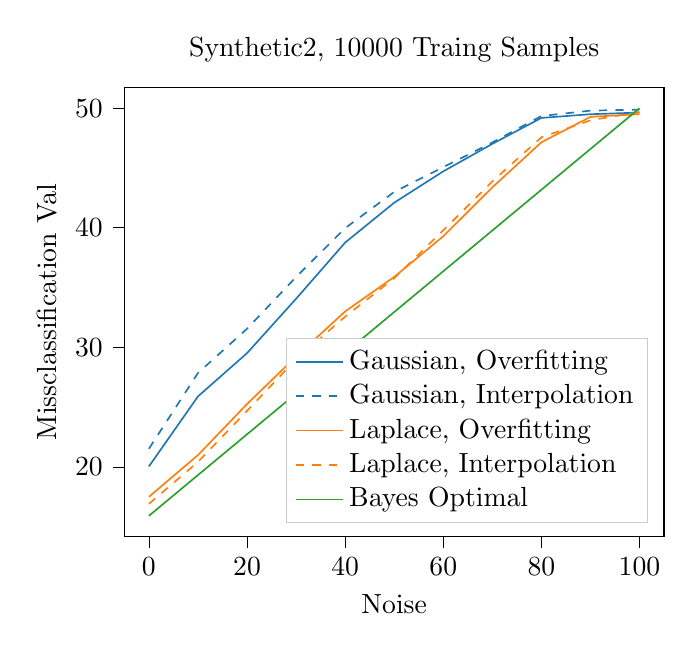
\begin{tikzpicture}

\definecolor{color0}{rgb}{0.12156862745098,0.466666666666667,0.705882352941177}
\definecolor{color1}{rgb}{1,0.498039215686275,0.0549019607843137}
\definecolor{color2}{rgb}{0.172549019607843,0.627450980392157,0.172549019607843}

\begin{axis}[
legend cell align={left},
legend style={at={(0.97,0.03)}, anchor=south east, draw=white!80.0!black},
tick align=outside,
tick pos=left,
title={Synthetic2, 10000 Traing Samples},
x grid style={white!69.01960784313725!black},
xlabel={Noise},
xmin=-5, xmax=105,
xtick style={color=black},
y grid style={white!69.01960784313725!black},
ylabel={Missclassification Val},
ymin=14.195, ymax=51.705,
ytick style={color=black}
]
\addplot [semithick, color0]
table {%
0 20.03
10 25.89
20 29.51
30 34.06
40 38.76
50 42.1
60 44.72
70 47.02
80 49.19
90 49.5
100 49.64
};
\addlegendentry{Gaussian, Overfitting}
\addplot [semithick, color0, dashed]
table {%
0 21.51
10 27.85
20 31.55
30 35.88
40 39.97
50 43
60 45.07
70 47.14
80 49.35
90 49.8
100 49.89
};
\addlegendentry{Gaussian, Interpolation}
\addplot [semithick, color1]
table {%
0 17.49
10 20.98
20 25.25
30 29.23
40 33
50 35.89
60 39.29
70 43.38
80 47.15
90 49.28
100 49.51
};
\addlegendentry{Laplace, Overfitting}
\addplot [semithick, color1, dashed]
table {%
0 16.9
10 20.41
20 24.68
30 29
40 32.56
50 35.78
60 39.79
70 43.88
80 47.57
90 48.99
100 49.69
};
\addlegendentry{Laplace, Interpolation}
\addplot [semithick, color2]
table {%
0 15.9
10 19.31
20 22.72
30 26.13
40 29.54
50 32.95
60 36.36
70 39.77
80 43.18
90 46.59
100 50
};
\addlegendentry{Bayes Optimal}
\end{axis}

\end{tikzpicture}